\documentclass[submit]{harvardml}

\newboolean{solutionCopy}
\setboolean{solutionCopy}{false} % Toggle between solution copy and distro

\ifthenelse{\boolean{solutionCopy}}{
  \includeversion{solution}
}{
  \excludeversion{solution}
}

% Put in your full name and email address.
\name{Nathan Nakatsuka}
\email{cs181-s17-nathan-nakatsuka}

% List any people you worked with.
\collaborators{%
  Joseph Sedlak
}

% You don't need to change these.
\course{CS181-S17}
\assignment{Assignment \#2}
\duedate{5:00pm Feb 24th, 2017}

\usepackage[OT1]{fontenc}
\usepackage[colorlinks,citecolor=blue,urlcolor=blue]{hyperref}
\usepackage[pdftex]{graphicx}
\usepackage{subfig}
\usepackage{fullpage}
\usepackage{amsmath}
\usepackage{amssymb}
\usepackage{color}
\usepackage{todonotes}
\usepackage{listings}
\usepackage{common}
\usepackage{bm}

\usepackage[mmddyyyy,hhmmss]{datetime}

\definecolor{verbgray}{gray}{0.9}

\lstnewenvironment{csv}{%
  \lstset{backgroundcolor=\color{verbgray},
  frame=single,
  framerule=0pt,
  basicstyle=\ttfamily,
  columns=fullflexible}}{}

\begin{document}


%%% Change the assignment details here:

\ifthenelse{\boolean{solutionCopy}}{
\begin{center}
{\Large \textbf{SOLUTION - Do Not Distribute}\\Homework 2: Bayesian Methods and Multiclass Classification}\\
\end{center}
}{
  \begin{center}
{\Large Homework 2: Bayesian Methods and Multiclass Classification}\\
\end{center}
}
\subsection*{Introduction}

This homework is about Bayesian methods 
and  multiclass classification. In lecture we have
primarily focused on binary classifiers trained to discriminate
between two classes. In multiclass classification, we discriminate
between three or more classes. We encourage you to first read the
Bishop textbook coverage of these topic, particularly: Section 4.2
(Probabilistic Generative Models), Section 4.3 (Probabilistic
Discriminative Models).
%, and, if MLE is troublesome, review 
%the materal Section 1
%and lecture 3.

As usual, we imagine that we have the input matrix $\boldX \in
\reals^{n \times m}$ (or perhaps they have been mapped to some basis
$\bm{\Phi}$, without loss of generality) but our outputs are now
``one-hot coded''.  What that means is that, if there are~$c$ output
classes, then rather than representing the output label $y$ as an
integer~${1,2,\ldots,c}$, we represent $\boldy$ as a binary vector of
length~$c$. These vectors are zero in each
component except for the one corresponding to the correct label, and
that entry has a one.  So, if there are 7 classes and a particular
datum has label 3, then the target vector would be~${C_3 = [0,0,1,0,0,0,0]}$. 
If there are $c$ classes, the set of possible outputs is $\{C_1 \ldots C_c \} = \{C_k\}_{k=1}^c$.
Throughout the assignment we will assume
that output $\boldy \in \{C_k\}_{k=1}^c$.\\

The problem set has four problems: 
\begin{itemize}
\item In the first problem, you will explore the properties of Bayesian
estimation methods for the Bernoulli model as well as the special
case of Bayesian linear regression with a simple prior.
%
\item In the second problem, you will explore the properties of the softmax
function, which is central to 
the method of
multiclass logistic regression. 
%We will also see that the 
%softmax plays a key role in  neural networks. 
%
\item  In the third
problem, you will dive into  matrix algebra and the methods behind
generative multiclass classifications. You will extend the discrete classifiers  
that we see in  lecture to a Gaussian model.
%
\item Finally, in the fourth problem, you will implement 
 logistic regression as well as a generative classifier 
from close to scratch.
%
\end{itemize}

\newpage
\begin{problem}[Bayesian Methods, 10 pts]

  This question helps to build your understanding of the
  maximum-likelihood estimation (MLE) vs. maximum a posterior estimator
  (MAP) and posterior predictive estimator, first in the
  Beta-Bernoulli model and then in the linear regression setting.\\

First consider the Beta-Bernoulli model (and see lecture 5.) 
%
\begin{enumerate}
\item[1.] Write down the expressions for the MLE, MAP and posterior predictive
distributions, and for
a prior $\theta\sim Beta(4,2)$ on the
parameter of the Bernoulli,
and  with data $D= 0, 0, 1, 1, 0, 0, 0, 0, 1, 0, 1, 1,$ 
$1, 0, 1, 0$, plot 
the three different
estimates after each additional
sample.
%
\item[2.] Plot the posterior distribution (prior for 0 examples) on $\theta$ after 0, 4, 8, 12 and 16
examples. (Using whatever tools you like.)
%
\item[3.] Interpret the differences you see between the three different
estimators.
%
%note, initial skew is to large 1, but data has $\theta=0.4$
%
\end{enumerate}

Second, consider the Bayesian Linear Regression model, with
data $D=\{(\boldx_i,y_i)\}_{i=1}^n$, $\boldx_i\in\mathbb{R}^m$,
 $y_i\in\mathbb{R}$, and generative model 
%
$$
y_i\sim\mcN(\boldw^\top\boldx_i,\beta^{-1})
$$
for (known) precision $\beta$ (which is just the reciprocal
of the variance). Given this, the likelihood of the
data is $p(\boldy|\boldX,\boldw) = \mcN(\boldy|\boldX\boldw,\beta^{-1}\mathbf{I})$. Consider the special case of 
an isotropic (spherical) prior on weights, with
%
$$
p(\boldw)=\mcN(\boldw|\bold0,\alpha^{-1}\boldI)
$$

\begin{enumerate}
\item[4.] Justify when you might use this prior in practice.
%
\item[5.] Using the method in lecture of taking logs, expanding and pushing terms
that don't depend on $\boldw$ into a constant, and finally collecting
terms and completing the square, confirm that the posterior on
weights after data $D$ is $\boldw\sim\mcN(\boldw|\boldm_n,\boldS_n)$,
where
%
\begin{align*}
\boldS_n&=(\alpha\boldI+\beta\boldX^\top\boldX)^{-1}\\
\boldm_n&=\beta\boldS_n\boldX^\top\boldy
\end{align*}
\item[6.] Derive the special case
of the MAP estimator for this problem as the isotropic
prior becomes arbitrarily weak.
What does the MAP estimator reduce to?
%
\item[7.] What did we observe in lecture about this
estimator for the case where 
the prior is neither weak nor strong?
\end{enumerate}
\end{problem}

\subsubsection*{Solution}
1)\\
Bernoulli PMF:\\
$p(x|\theta)=\prod_{i=1}^{n}\theta^x(1-\theta)^{1-x}$\\
$\textrm{ln}(p(x|\theta))=n_1\textrm{ln}\theta+n_0\textrm{ln}(1-\theta)$
Setting the derivative (wrt $\theta$) to $0$, you get the expression for MLE (doesn't make use of prior): $\dfrac{n_1}{n_0+n_1}$
\\
$p(\theta|D) = \textrm{Beta}(\theta|n_1+\alpha,n_0+\beta)$. Therefore, expression for MAP:\\
$\theta_{\textrm{MAP}}=\dfrac{\alpha+n_a-1}{\alpha+\beta+n_1+n_0-2}$\\
Expression for Posterior Predictive Distribution:\\
$p(x=1|D) = \dfrac{\alpha+n_a}{\alpha+\beta+n_1+n_0}$.\\
See figure 1 for plot.
\\
\begin{figure}[h]
\centering
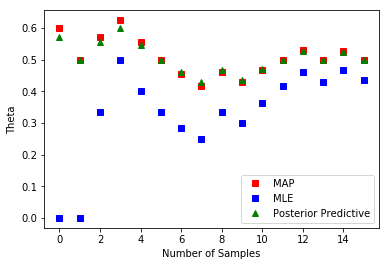
\includegraphics[width=0.8\textwidth]{h2_figure1}
\caption{Plot of MLE, MAP, and posterior predictive distributions for Bernoulli with a Beta prior after various amounts of data.}
\label{fig:1.1}
\end{figure}

2)\\
See Figure 2.\\
\begin{figure}[h]
\centering
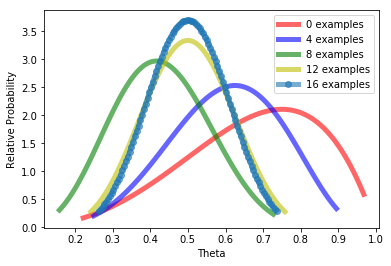
\includegraphics[width=0.8\textwidth]{h2_figure2}
\caption{Plot of Beta posterior after various amounts of data.}
\label{fig:1.1}
\end{figure}

3)\\
The MLE is purely based on the data, so it starts off with bad estimates until it gets enough data.  Since there are only 16 samples, the original beta prior retains an effect on the final estimate, causing the MAP and posterior predictive estimates to be larger than the MLE at all points.  The MAP estimate starts off higher than the posterior predictive, because it subtracts the equivalent of $1/2$ from the estimate, but after a few data points, the MAP and posterior predictive end up being essentially the same.
\\
4)\\
One might use an isotropic (spherical) prior if it is expected that the weights should be centered around 0 (example, random noise).  
\\
5)\\
$p(\textbf{w}|D) \propto N(\textbf{w}|0,\alpha^{-1}\textbf{I})N(\textbf{y}|\textbf{X}\textbf{w},\beta^{-1}\textbf{I}) = \dfrac{1}{|2\pi \alpha^{-1}\textbf{I}|}\exp(-\dfrac{1}{2}\textbf{w}^{\textrm{T}}\alpha^{-1}\textbf{I}\textbf{w}) \dfrac{1}{|2\pi \beta^{-1}\textbf{I}|}\exp(-\dfrac{1}{2}(\textbf{y}-\textbf{X}\textbf{w})^{\textrm{T}}\beta^{-1}\textbf{I}(\textbf{y}-\textbf{X}\textbf{w}))$\\
$\textrm{ln} p(\textbf{w}|D) = \textrm{Constant} - \dfrac{1}{2}[\textbf{w}^{\textrm{T}}\alpha^{-1}\textbf{I}\textbf{w}) + (\textbf{y}-\textbf{X}\textbf{w})^{\textrm{T}}\beta^{-1}\textbf{I}(\textbf{y}-\textbf{X}\textbf{w})]$\\
$\textrm{ln} p(\textbf{w}|D) = \textrm{Constant} - \dfrac{1}{2}(\textbf{w}^{\textrm{T}}(\alpha\textbf{I}+\beta \textbf{X}^{\textrm{T}}\textbf{X})\textbf{w}-2\textbf{w}^{\textrm{T}}(\beta\textbf{X}^{\textrm{T}}\textbf{y}))$\\
Complete the square:\\
$\textrm{ln} p(\textbf{w}|D) = \textrm{Constant} - \dfrac{1}{2}a (\textbf{w}-b/a)^2$, where $a=(\alpha\textbf{I}+ \beta \textbf{X}^{\textrm{T}}\textbf{X})$, and $b=(\beta\textbf{X}^{\textrm{T}}\textbf{y})$\\
Then $\textbf{S}_n=a=(\alpha\textbf{I}+ \beta \textbf{X}^{\textrm{T}}\textbf{X})^{-1}$, and
$\textbf{m}_n=b/a=(\beta \textbf{S}_n \textbf{X}^{\textrm{T}}\textbf{y})$.\\
This matches the normal distribution with mean of $\textbf{m}_n$ and variance of $\textbf{S}_n$.
\\
6)\\
If the prior becomes very weak, that means $\alpha$ is very large, so the MAP estimator, which is $\textbf{m}_n=\dfrac{(\beta \textbf{X}^{\textrm{T}}\textbf{y})}{(\alpha\textbf{I}+ \beta \textbf{X}^{\textrm{T}}\textbf{X})}$, reduces to the MLE, which is $\dfrac{\textbf{y}}{\textbf{X}}$.

7)\\
If the prior is neither weak nor strong, it becomes the regularization constant of LASSO.




\newpage
%\subsection*{1. Properties of Softmax [5pts]}
%%%%%%%%%%%%%%%%%%%%%%%%%%%%%%%%%%%%%%%%%%%%%
% Problem 1
%%%%%%%%%%%%%%%%%%%%%%%%%%%%%%%%%%%%%%%%%%%%%
\begin{problem}[Properties of Softmax, 8pts]
%
  We have explored logistic regression, which is a discriminative
  probabilistic model over two classes. For each input $\boldx$,
  logistic regression outputs a probability of the class output $y$
  using the logistic sigmoid function.

  The softmax transformation is an important generalization of the logistic
  sigmoid to the case of $c$ classes. It takes as input a vector, and
  outputs a transformed vector of the same size,
%
  \[ \mathrm{softmax}(\boldz)_k =\frac{\exp(z_k)}{\sum_{\ell=1}^c \exp(z_{\ell})}, \ \ \text{for all $k$}\]

Multiclass logistic regression uses the softmax transformation over vectors of size $c$. Let $\{\boldw_{\ell}\} = \{\boldw_1 \ldots \boldw_c \} $
denote the parameter vectors for each class.
In particular,  multiclass logistic regression 
defines the probability of class $k$ as,
%
\begin{align*}
  p(\boldy=C_k \given \boldx; \{\boldw_{\ell}\})
  &= \mathrm{softmax}([\boldw_1^{\top}\boldx \ldots \boldw_c^{\top} \boldx]^\top)_k =  \frac{ \exp( \boldw_k^{\top}\boldx ) }
  {  \sum_{\ell=1}^c \exp( \boldw_{\ell}^{\top}\boldx ) }\,.
\end{align*}

\noindent  As above, we are
using~$\boldy = {C_{k}}$ to indicate the output 
vector that represents class $k$.

Assuming data $D = \{(\boldx_i, \boldy_i)\}_{i=1}^n$,
the negated log-likelihood  can be written in the standard form, as
%
\[\mcL(\{\boldw_{\ell}\}) = - \sum_{i=1}^n \ln  p(\boldy_i \given \boldx_i; \{\boldw_{\ell}\}) \]


Softmax is an important function in the context of machine learning,
and you will see it again in other models, such as neural networks.
In this problem, we aim to gain intuitions into the properties of
softmax and multiclass logistic regression.

Show that:
\begin{enumerate}
  \item The output of the softmax function is a vector with non-negative components
    that are at most 1. 
%
  \item The output of the softmax function defines a distribution,
so that in addition, the components sum to 1.
%
  \item Softmax preserves order. This means that if elements $z_k < z_\ell$,
in $\boldz$, then  $\mathrm{softmax}(\boldz)_k < \mathrm{softmax}(\boldz)_{\ell}$ for any $k,\ell$. 
  \item Show that \[\frac{\partial \mathrm{softmax}(\boldz)_k }{\partial z_j} = \mathrm{softmax}(\boldz)_k (I_{kj} - \mathrm{softmax}(\boldz)_j) \ \ \text{for\ any\ } k, j  \],
%
where indicator $I_{kj}=1$ if $k=j$ and $I_{kj}=0$ otherwise.
%
  \item Using your answer to the previous question, show that
    \[ \frac{\partial }{\partial \boldw_k} \mcL(\{\boldw_{\ell}\}) = \sum_{i=1}^n (p(\boldy_i = C_k | \boldx_i; \{\boldw_\ell\}) - y_{ik} ) \boldx_i  \]
    By the way, this may be useful for Problem 3!
\end{enumerate}
\end{problem}


\subsubsection*{Solution}
1)\\
Given the softmax is purely using exponential functions, all of these functions give non-negative outputs, so the softmax function output must be non-negative.  Since, the numerator is a subset of the denominator, the output can only be at most 1.\\
2)\\
If you sum up the numerator of the softmax function, it will equal the denominator, which is a sum of all of the elements of the vector $\textbf{w}$.  Thus, the components sum to 1.  This is a distribution, because it gives values corresponding to each datapoint.\\
3)\\
The denominator for each of the softmax functions for a particular vector of values will be the same, and if $z_k < z_l$, then the numerator term of softmax($\textbf{z}$)$_k$ will be less than the numerator of softmax($\textbf{z}$)$_l$, so softmax($\textbf{z}$)$_k$ will be less than softmax($\textbf{z}$)$_l$ for any $k$,$l$.\\
4)\\
$\frac{\partial \exp{(\textbf{w}_k^{\textrm{T}}\textbf{x})}}{\partial z_j\sum_{l=1}^{c}\exp{(\textbf{w}_l^{\textrm{T}}\textbf{x})}} =$ \\
\\
If $k=j$:\\
$\dfrac{(\textbf{w}_k^{\textrm{T}}\textbf{x})*\exp{(\textbf{w}_k^{\textrm{T}}\textbf{x})}*(\sum_{l=1}^{c}\exp{(\textbf{w}_l^{\textrm{T}}\textbf{x})})-\exp{(\textbf{w}_k^{\textrm{T}}\textbf{x})}*((\textbf{w}_k^{\textrm{T}}\textbf{x})*\exp{(\textbf{w}_k^{\textrm{T}}\textbf{x})})}{(\sum_{l=1}^{c}\exp{(\textbf{w}_l^{\textrm{T}}\textbf{x})})^2}$\\
$=$ softmax($\textbf{z}$)$_k(\dfrac{\sum_{l=1}^{c}\exp{(\textbf{w}_l^{\textrm{T}}\textbf{x})}-\exp{(\textbf{w}_l^{\textrm{T}}\textbf{x})}}{\sum_{l=1}^{c}\exp{(\textbf{w}_l^{\textrm{T}}\textbf{x})}})=$ softmax($\textbf{z}$)$_k(I_{kj}-$softmax($\textbf{z}$)$_k$)\\
\\
If $k !=j$:\\
$\dfrac{-\exp{(\textbf{w}_k^{\textrm{T}}\textbf{x})}*(\exp{(\textbf{w}_j^{\textrm{T}}\textbf{x})})}{(\sum_{l=1}^{c}\exp{(\textbf{w}_l^{\textrm{T}}\textbf{x})})^2}=$ softmax($\textbf{z}$)$_k*(-$softmax($\textbf{z}$)$_k$)

(noting that the components sum to 1).\\
\\
5)\\
$\dfrac{\partial}{\partial \textbf{w}_k}L({\textbf{w}_l}) = -\sum_{i=1}^{n}\dfrac{p(y|x_{i};\left\{ \textbf{w}_l \right\})(I_{kj}-p(y|x_{i};\left\{ \textbf{w}_l \right\}))}{p(y|x_{i};\left\{ \textbf{w}_l \right\})}$\\
The indicator variable becomes a one-hot matrix over all classes and thus becomes $y_{ik}*\textbf{x}_i$.  Thus, the expression becomes:\\

$=$
$\sum_{i=1}^{n}(p(y|x_{i};\left\{ \textbf{w}_l \right\})-I_{kj})$
$=$
$\sum_{i=1}^{n}(p(y|x_{i};\left\{ \textbf{w}_l \right\})-y_{ik})\textbf{x}_i$





%\subsection*{2. Mooooar matrix calculus [10 pts]}
%%%%%%%%%%%%%%%%%%%%%%%%%%%%%%%%%%%%%%%%%%%%%
% Problem 2
%%%%%%%%%%%%%%%%%%%%%%%%%%%%%%%%%%%%%%%%%%%%%
\begin{problem}[Return of matrix calculus, 10pts]

  Consider now a generative $c$-class model.  We adopt class prior
  $p(\boldy = C_k; \bpi) = \pi_k$ for all $k \in \{1, \ldots, c\}$
(where $\pi_k$ is a parameter of the prior).
%
%that define the prior. 
Let  $p(\boldx|\boldy=C_k)$ denote
the class-conditional density of features $\boldx$ (in this
case for class $C_k$). Consider the data set $D = \{(\boldx_i,
\boldy_i)\}_{i=1}^n$ where as above $\boldy_i \in \{C_k\}_{k=1}^c$ is
encoded as a one-hot target vector. 
%
\begin{enumerate}
  \item Write out the negated log-likelihood of the data set,
    $-\ln p(D ; \bpi)$.
%
  \item Since the prior forms a distribution, it has the constraint that
    $\sum_k\pi_k - 1 = 0$.  Using the hint on
Lagrange multipliers below, give the
    expression for the maximum-likelihood estimator for the prior
    class-membership probabilities, i.e.
    $\hat \pi_k.$
    Make sure to write out the intermediary equation you need
    to solve to obtain this estimator. Double-check your answer: the final
    result should be very intuitive!
\end{enumerate}

    For the remaining questions, let the 
    class-conditional probabilities be Gaussian distributions with 
the same covariance matrix
    $$p(\boldx | \boldy = C_k) = \mathcal{N}(\boldx |  \bmu_k, \bSigma), \text{\ for\ }k \in \{1,\ldots, c\}$$
%
and different means $\bmu_k$ for each class.
%
    \begin{enumerate}
  \item[3.] Derive the gradient of the negative log-likelihood with respect to vector $\bmu_k$.
    Write the expression in matrix form as a function of the variables defined
    throughout this exercise. Simplify as much as possible for full credit.
  \item[4.] Derive the maximum-likelihood estimator for vector $\bmu_k$. Once
    again, your final answer should seem intuitive.
  \item[5.] Derive the gradient for the negative log-likelihood with respect to the
    covariance matrix $\bSigma$ (i.e., looking
to find an MLE for the covariance). 
Since you are differentiating with respect to a
    \emph{matrix}, the resulting expression should be a matrix!
%
  \item[6.] Derive the maximum likelihood estimator of the covariance matrix.
\end{enumerate}

\paragraph{[Hint: Lagrange Multipliers.} Lagrange Multipliers are a method for
optimizing a function $f$ with respect to an
equality constraint, i.e. 
\[\min_{\boldx} f(\boldx)\ \text{s.t.}\ g(\boldx) = 0.\]

This can be turned into an unconstrained problem by introducing a
Lagrange multiplier $\lambda$ and constructing the Lagrangian function,
\[L(\boldx, \lambda) =  f(\boldx) + \lambda g(\boldx).\]

It can be shown that it is a necessary condition that the optimum 
is a critical point of this new function. We can find this point by solving two equations:

\[\frac{\partial L(\boldx, \lambda)}{\partial  \boldx} = 0  \ \ \text{and}\  \  \frac{\partial L(\boldx, \lambda)}{\partial \lambda} = 0 \]


\paragraph{Cookbook formulas.} Here are some formulas you might want to consider
using to compute difficult gradients. You can use them  in the homework
without proof. If you are looking to hone your matrix calculus skills, try to
find different ways to prove these formulas yourself (will not be part of the
evaluation of this homework). In general, you can use any formula from the matrix cookbook,
as long as you cite it. We opt for the following common notation:
$\boldX^{-\top} := (\boldX^{\top})^{-1}$
\begin{align*}
  & \frac{\partial \bolda^\top \boldX^{-1} \boldb}{\partial \boldX} = - \boldX^{-\top} \bolda \boldb^\top \boldX^{-\top} \\
  & \frac{\partial \ln | \det (\boldX) |}{\partial \boldX} = \boldX^{-\top}
 \end{align*}
 \end{problem}



\subsubsection*{Solution}
1)\\
This can be modeled in part as a multinomial distribution, so:
$p(D; \boldsymbol{\pi})= \prod_{i=1}^{n}\prod_{k=1}^{c}(\boldsymbol{\pi}_k p(\textbf{x}|\textbf{y}=C_k))^{yk}$

$-\textrm{ln} p(D; \boldsymbol{\pi})= \sum_{i=1}^{n}\sum_{k=1}^{c}-(\textrm{ln} (\boldsymbol{\pi}_k) + \textrm{ln} p(\textbf{x}|\textbf{y}=C_k))*(yk)$\\

2)\\
From above, we know that the negative log likelihood of the prior is:\\
$-\sum_{i=1}^{n}\sum_{k=1}^{c}(y_{ik}\textrm{ln}\pi_k)$\\
Optimizing the function with respect to the constraint gives:\\
$L(\pi,\lambda) = -\sum_{i=1}^{n}\sum_{k=1}^{c}(y_{ik}\textrm{ln}\pi_k) + \lambda(1-\sum_{k=1}^{c}(\pi_k))$\\
To attain the optimum of this function, we must solve the two equations setting the derivatives with respect to $\pi_k$ and $\lambda$ to 0:\\
$\frac{\partial L(\pi,\lambda)}{\partial \pi_k}= 0 = -\sum_{i=1}^{n}\dfrac{y_{ik}}{\pi_k} -\lambda$ \\
$\frac{\partial L(\pi,\lambda)}{\partial \lambda}= 0 = 1-\sum_{k=1}^{c}(\pi_k)$ \\
Using these 2 equations, we see that:\\
$\lambda = n$ and $\hat{\pi} = \dfrac{\sum_{i=1}^{n}(y_{ik})}{\sum_{i=1}^{n}\sum_{k=1}^{c}(y_{ik})}$\\
This essentially means that the prior for each class is the total number of objects in that class divided by the total number of objects in all classes.\\

3)\\
$-\textrm{ln}p(\textbf{x}|\textbf{y} = C_k) =  Constant + \dfrac{1}{2}\sum_{k=1}^{c}(\textbf{x}-\mu_k)^{\textrm{T}}\Sigma^{-1}(\textbf{x}-\mu_k)$\\
$=\dfrac{1}{2}\sum_{k=1}^{c}(\mu_k^{\textrm{T}}\Sigma^{-1}\mu_k + \textbf{x}^{\textrm{T}}\Sigma^{-1}\textbf{x} + 2\textbf{x}^{\textrm{T}}\Sigma^{-1}\mu_k)$\\
$-\frac{\partial \textrm{ln}p(\textbf{x}|\textbf{y})}{\partial \mu_k} =  \sum_{k=1}^{c}(\mu_k^{\textrm{T}}\Sigma^{-1} + \textbf{x}^{\textrm{T}}\Sigma^{-1})$

4)\\
$-\frac{\partial \textrm{ln}p(\textbf{x}|\textbf{y})}{\partial \mu_k} = 0 => \hat{\mu_k} = \dfrac{\sum_{i=1}^{n}\textbf{x}_{ik}}{n_k}$
This means that the MLE for $\mu_k$ is the sum of the observations for a given class divided by the total number of observations in that class.


5/6)\\
$-\textrm{ln}p(\textbf{x}|\textbf{y} = C_k) =  Constant + \dfrac{N}{2}\textrm{ln}|\Sigma| + \dfrac{1}{2}\sum_{k=1}^{c}(\textbf{x}-\mu_k)^{\textrm{T}}\Sigma^{-1}(\textbf{x}-\mu_k)$\\
$-\textrm{ln}p(\textbf{x}|\textbf{y} = C_k) =  Constant + \dfrac{N}{2}\textrm{ln}|\Sigma| + \dfrac{1}{2}tr(\Sigma^{-1}\sum_{k=1}^{c}(\textbf{x}-\mu_k)^{\textrm{T}}(\textbf{x}-\mu_k))$\\
From matrix cookbook:\\

$-\frac{\partial \textrm{ln}p(\textbf{x}|\textbf{y})}{\partial \Sigma} =  \dfrac{N}{2}\Sigma^{-\textrm{T}} + \dfrac{1}{2}\Sigma^{\textrm{T}}\sum_{k=1}^{c}(\textbf{x}-\mu_k)^{\textrm{T}}(\textbf{x}-\mu_k))$\\
$-\frac{\partial \textrm{ln}p(\textbf{x}|\textbf{y})}{\partial \Sigma} = 0 => \hat{\Sigma} = \dfrac{1}{N}\sum_{k=1}^{c}(\textbf{x}-\mu_k)^{\textrm{T}}(\textbf{x}-\mu_k)$






\newpage
\subsection*{4. Classifying Fruit [15pts]}
You're tasked with  classifying three different kinds of fruit, based on their
heights and widths.  Figure~\ref{fig:fruit} is a plot of the data.  Iain Murray
collected these data and you can read more about this on his website at
\url{http://homepages.inf.ed.ac.uk/imurray2/teaching/oranges_and_lemons/}.  We
have made a slightly simplified (collapsing the subcategories together) version
of this available as \verb|fruit.csv|, which you will find in the Github repository.
The file has three columns: type (1=apple, 2=orange, 3=lemon), width,
and height.  The first few lines look like this:
\begin{csv}
fruit,width,height
1,8.4,7.3
1,8,6.8
1,7.4,7.2
1,7.1,7.8
...
\end{csv}
\begin{figure}[h]
\centering
\includegraphics[width=0.5\textwidth]{fruit}
\caption{Heights and widths of apples, oranges, and lemons.  These fruit were
purchased and measured by Iain Murray:
\url{http://homepages.inf.ed.ac.uk/imurray2/teaching/oranges_and_lemons/}.}
\label{fig:fruit}
\end{figure}
\begin{problem}[Classifying Fruit, 15pts]
You should implement the following:
\begin{itemize}
\item The three-class generalization of logistic regression, also
  known as softmax regression, for these data. You will do this by implementing
  gradient descent on the negative log likelihood. You will need to find good values for the learning rate $\eta$ and regularization strength $\lambda$.
%
\item A generative classifier with Gaussian
  class-conditional densities, as in Problem~3. In particular, make
  two implementations of this, one with a shared covariance matrix
  across all of the classes, and one with a separate covariance being
  learned for each class.  Note that the staff implementation can
  switch between these two by the addition of just a few lines of
  code. In the separate covariance matrix case, the MLE for the
  covariance matrix of each class is simply the covariance of the data
  points assigned to that class, without combining them as in the
  shared case.
\end{itemize}
You may use anything in  \texttt{numpy} or \texttt{scipy}, except for \texttt{scipy.optimize}. That being said, if you happen to find a function in \texttt{numpy} or \texttt{scipy} that seems like it is doing too much for you, run it by a staff member on Piazza. In general, linear algebra and random variable functions are fine. The controller file is \texttt{problem4.py}, in which you will specify hyperparameters. The actual implementations you will write will be in \texttt{LogisticRegression.py} and \texttt{GaussianGenerativeModel.py}.


You will be given class interfaces for \texttt{GaussianGenerativeModel} and \texttt{LogisticRegression} in the distribution code, 
and the code will indicate certain lines that you should not change in your final submission. Naturally, don't change these.
These classes will allow the final submissions to have consistency. There will also be a few hyperparameters that are set to
irrelevant values at the moment. You may need to modify these to get your methods to work.
The classes you implement follow the same pattern as scikit-learn, so they should be familiar to you. The distribution code currently outputs nonsense predictions just to show what the high-level interface should be, so you should completely remove the given \texttt{predict()} implementations and replace them with your implementations.

\begin{itemize}
\item The \texttt{visualize()} method for each classifier will save a plot that will show the decision boundaries. You should include these in this assignment.
\item Which classifiers model the distributions well?
\item What explains the differences?

\end{itemize}

In addition to comparing the decision bounadaries of the three models visually:
\begin{itemize}

\item For logistic regression, report negative log-likelihood loss for several configurations of hyperparameters. Why are your final choices of learning rate ($\eta$) and regularization strength ($\lambda$) reasonable? Plot loss during training for the best of these configurations, with iterations on the x-axis and loss on the y-axis (one way to do this is to add a method to the LogisticRegression Class that displays loss).

\item For both Gaussian generative models, report likelihood. In the separate covariance matrix case, be sure to use the covariance matrix that matches the true class of each data point.

\end{itemize}

\end{problem}

\subsubsection*{Solution}
1)\\
The Gaussian generative model with separate co-variance matrices models the distributions the best.  This is because it can form non-linear boundaries.  The model with separate co-variance matrices is better than the one that assumes the same co-variance matrices, because the actual underlying distributions have different co-variances.  \\
In Table 1 I report different negative log-likelihood losses for different hyperparameters.  The final choices are reasonable, because at a certain point the eta value will not affect much, but it slows down the algorithm to have a lower value.  The lambda value I chose (.1) had slightly higher loss than 1, but this was due to the outliers of the blue points.  Otherwise, it got closer to the red points, and would have been better for future predictions.\\
For the Gaussian Generative Model with separate covariance matrices, the likelihood was -158.1, and for the model with shared covariance matrices, the likelihood was -185.3.


\begin{figure}[h]
\centering
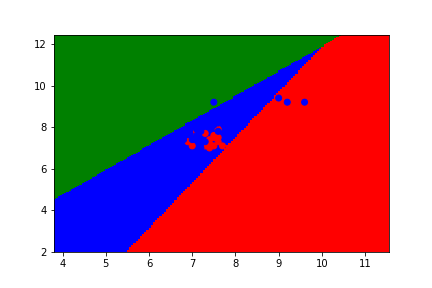
\includegraphics[width=0.8\textwidth]{logistic_regression_result}
\caption{Plot of logistic regression classifier decision boundaries.}
\label{fig:1.3}
\end{figure}

\begin{table}
\centering
\begin{tabular}{llr}
 %\toprule
 \multicolumn{2}{c}{Scores} \\
 Eta & Lambda & Negative Log-Likelihood Score \\
% \midrule
 0.1 & 0.1 & 4744.9\\
 0.001 & 0.1 & 34.8 \\
 0.0001 & 0.1 & 25.8  \\
 0.0001 & 10 & 33.9  \\
 0.0001 & 1 & 22.3  \\
 0.0001 & 0.1 & 25.8  \\
 0.0001 & 0.01 & 28.2  \\
 %\bottomrule
\end{tabular}
\caption{\label{tab:results} Negative log-likelihood scores for different hyperparameters.}
\end{table}


\begin{figure}[h]
\centering
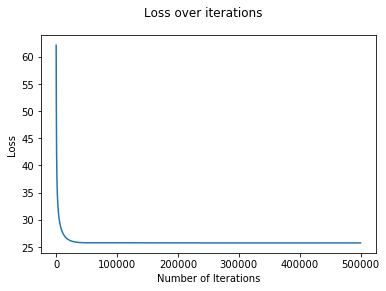
\includegraphics[width=0.8\textwidth]{h2_figure4}
\caption{Plot of loss over many iterations in logistic regression classifier.}
\label{fig:1.4}
\end{figure}

\begin{figure}[h]
\centering
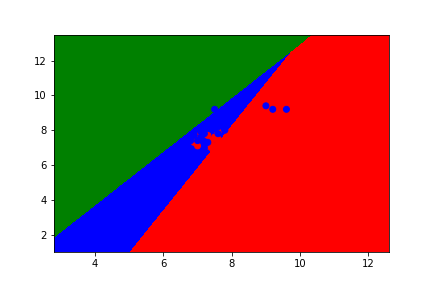
\includegraphics[width=0.8\textwidth]{generative_result_shared_covariances}
\caption{Plot of Gaussian Generative Model classifier decision boundaries with shared covariance matrix.}
\label{fig:1.5}
\end{figure}

\begin{figure}[h]
\centering
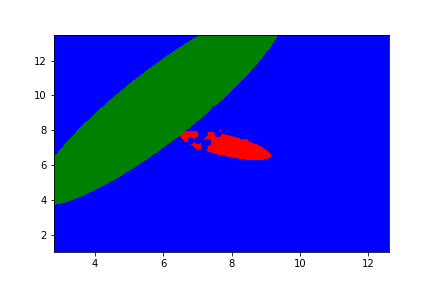
\includegraphics[width=0.8\textwidth]{generative_result_separate_covariances}
\caption{Plot of Gaussian Generative Model classifier decision boundaries with separate covariance matrix.}
\label{fig:1.6}
\end{figure}



\newpage
\subsection*{Calibration [1pt]}
Approximately how long did this homework take you to complete?
20 hours

\end{document}
